\section{Introduzione}
Nella terza iterazione è stato approfondito e implementato l'algoritmo portante del sistema: l'algoritmo di Discover permette di ``Scoprire" nuova 
musica e nuovi utenti in base alle preferenze dell'utente.


\section{Descrizione dell'algoritmo}
L'algoritmo di Discover è stato ideato per offrire all'utente un'esperienza completa di riproduzione e scoperta di nuova musica, unendo a ciò la 
componente social: in questo modo si permette all'utente di conoscere nuove persone che condividono con lui i propri gusti musicali. 

Questo tipo di algoritmo 
tiene traccia dei generi preferiti dell'utente e lo utilizza per suggerire musica simile, ma non solo: allo stesso modo riesce a suggerire 
una lista di utenti che hanno gusti simili all'utente loggato, in modo da poterli aggiungere alla propria lista di amici.  

Le variabili e i fattori tenuti in considerazione per lo sviluppon dell'algoritmo di Discover sono i seguenti: 
\begin{itemize}
    \item Il genere favorito dell'utente, ottenuto da un'analisi dei suoi brani preferiti;
    \item L'età dell'utente;
    \item Il sesso dell'utente.
\end{itemize}


\newpage
\section{Funzionamento dell'algoritmo}
Il funzionamento dell'algoritmo si basa su una previsione Machine Learning, tramite la libreria \textbf{Pandas} di Python;
il nome fa riferimento sia a ``Panel Data" che ``Python Data Analysis", infatti è una libreria molto utilizzata per lavorare 
con dataset: tramite le sue molteplici funzioni consente di analizzare, pulire, esplorare e manipolare i dati, definendo 
conclusioni basate su teorie statistiche. 

Come anticipato, in base al genere preferito dell'utente, il suo sesso e la sua età, l'algoritmo suggerisce dei brani ricavandoli 
da un dataset, filtrandoli secondo le variabili sopracitate. Al termine dell'esecuzione l'algoritmo mostrerà un elenco di brani e amici suggeriti.

Gli step di funzionamento dell'algoritmo possono essere così riassunti: 
\begin{itemize}
    \item Inizialmente, viene creato un oggetto account contenente le informazioni relative all'account dell'utente loggato, che ci serviranno in seguito; 
    viene passato il parametro \textbf{request} che è quello che contiene le informazioni di interesse, ovvero l'età e il sesso (1=maschio, 0=femmina). 
    In seguito viene utilizzato un training set (\textbf{utenti.csv}) sul quale allenare la stima, contenente le informazioni degli utenti 
    necessarie per estrapolare le variabili: quelle di input includono il sesso e l'età dell'utente, quella di output contiene solo 
    il genere preferito (ciò che suggerirà l'algoritmo). 

    \item Dopo aver creato queste due tabelle viene istanziato il modello previsionale tramite il comando \textbf{DecisionTreeClassifier}, un comando 
    della libreria Pandas che permette, dandogli in input le variabili considerate, di fittare il modello che le lega. 
    
    \item Viene quindi fittato il modello tramite il comando \textbf{modello.fit(...)}, che si allenerà sulle variabili scelte (età e sesso), per restituire 
    il risultato (genere preferito). 

    \item In seguito verrà effettuata la predizione inserendo le informazioni relative all'utente loggato tramite la funzione \textbf{modello.predict}, ed 
    infine viene memorizzata la previsione relativa solo alla variabile di genere musicale. 
    
\end{itemize}


\newpage
\subsection{Discover: Suggerimento brano}
Nella parte successiva dell'algoritmo Discover si effettua un semplice filtro su tutte le canzoni presenti nel database del sistema e vengono
 selezionate solo quelle che rispettano il genere target restituito dall'algoritmo Discover; vengono in seguito salvate in una 
 lista e proposte all'utente, che sarà in grado di navigare e selezionare quale scaricare o aggiungere ai preferiti o ad una playlist. 

\subsection{Discover: Suggerimento amici}
Nell'ultima parte dell'algoritmo Discover viene seguito un processo più meccanico: facendo ancora riferimento al genere target 
individuato nella parte iniziale dell'algoritmo, viene estrapolata una lista di amici suggeriti per l'utente. 

Inizialmente viene creata una lista amici vuota, vengono salvate le informazioni relative dell'utente loggato, vengono quindi 
selezionati tutti gli utenti presenti nella lista amici (in modo da escluderli in seguito nell'algoritmo).
Dopo aver creato una lista degli identificativi, tramite un ciclo for each vengono selezionati gli utenti nel database 
sfogliando per ognuno le canzoni preferite, al fine di salvare il genere di ogni canzone in una variabile y.

Condizione per rientrare negli utenti suggeriti:
\begin{itemize}
    \item L'utente analizzato (nel database) non deve essere l'utente loggato, ovvero devono avere id diversi;
    \item L'utente analizzato (nel database) non deve essere amico dell'utente loggato, ovvero il suo id non deve essere presente 
    nella lista amici;
    \item All'utente analizzato (nel database) deve piacere almeno una canzone che abbia lo stesso genere target dell'algoritmo.

\end{itemize}

Nel context viene poi passata la lista creata con gli utenti selezionati dal database, in modo da permettere all'utente di poter
navigare fra gli utenti ed, eventualmente, aggiungerli fra gli amici. 

\subsection{Bootstrap}
Per il frontend è stato utilizzato Bootstrap, un framework per frontend e web development semplice e veloce. 
Bootstrap include templates design basati su HTML e CSS per tipografia, forme, pulsanti, tabelle, navigazione, caroselli di 
immagini e molto altro, come anche plugin opzionali di JavaScript; è' molto semplice da usare e possiede un'alta 
compatibilità con i browser maggiormente usati. 


\section{Studio della complessità}


\subsection{Pseudocodice}

Pseudocodice parte iniziale algoritmo. 
\begin{figure}[H]
    \centering
    \begin{center}
    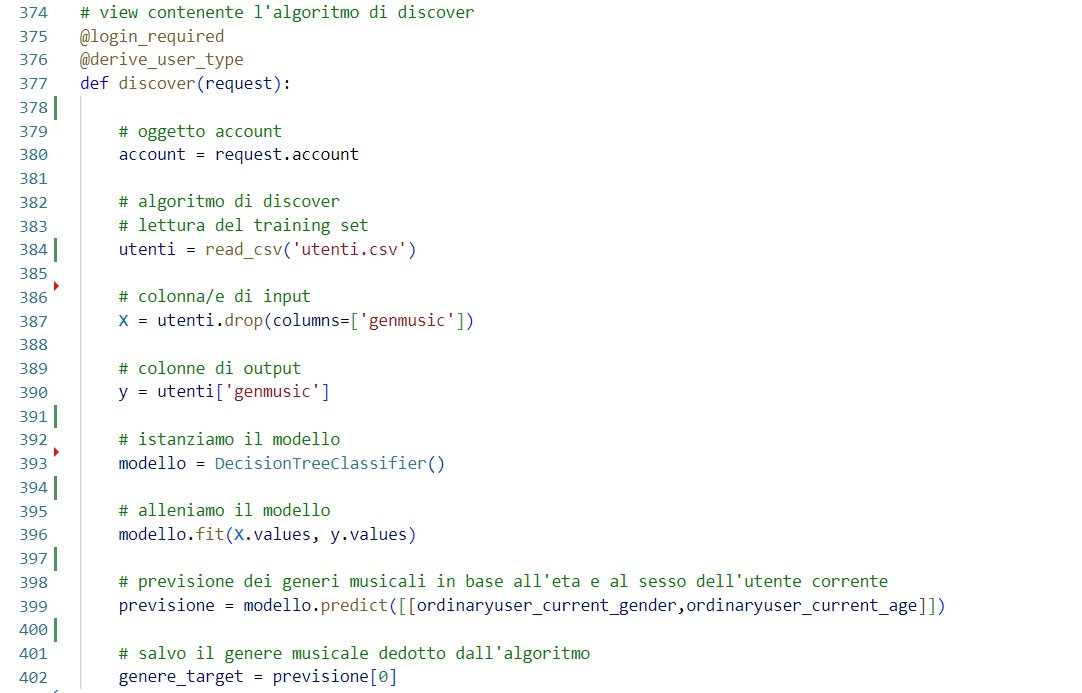
\includegraphics[scale=0.7]{images/alg1.jpg}
    \end{center}
    \caption{Pseudocodice}
    \label{fig-pseudocodice-1}
\end{figure}




% algoritmo 1
\begin{algorithm}[H]
    \caption{Step 1 - Inizializzazione}
    \SetAlgoLined
    \LinesNumbered
    \SetKwProg{myalg}{algoritmo}{ begin}{end}
    \myalg{Discover($curruser\_gender$, $curruser\_age$)}{
        \BlankLine
        \BlankLine
        \textbf{/* Creazione oggetto account */}\

        \textbf{do}{
            $account \leftarrow request.account$
        }
        \BlankLine
        \BlankLine
        \textbf{/* Lettura training set degli utenti.csv */}\
            
        \textbf{do}{
           $utenti \leftarrow read\_csv('utenti.csv')$
        }
        \BlankLine
        \BlankLine
        \textbf{/* Creazione colonna di input della previsione */}\
            
        \textbf{do}{
            $X \leftarrow utenti.drop(columns=['genmusic'])$
        }
        \BlankLine
        \BlankLine
        \textbf{/* Creazione colonna di output della previsione */}\
            
        \textbf{do}{
            $y \leftarrow utenti['genmusic'] $
        }
        \BlankLine
        \BlankLine
        \textbf{/* Creazione istanza del modello */}\
            
        \textbf{do}{
            $ modello \leftarrow \underline{DecisionTreeClassifier()}$
        }
        \BlankLine
        \BlankLine
        \textbf{/* Allenamento del modello sui dati */}\
            
        \textbf{do}{
            $ modello.\underline{fit}(X.values, y.values)$
        }
        \BlankLine
        \BlankLine
        \textbf{/* Previsione dei generi */}\
            
        \textbf{do}{
            $previsione \leftarrow modello.\underline{predict}(curruser\_gender, curruser\_age)$
        }
        \BlankLine
        \BlankLine
        \textbf{/* Memorizzazione del genere target */}\

        \textbf{do}{
            $genere\_target \leftarrow previsione[0]$
        } 

        \BlankLine
        \BlankLine
        \KwResult{Genere target}
        \BlankLine
        \BlankLine
        \textbf{...} \vspace{0.5cm}
        %\label(Step 1 - Inizializzazione)
        %\ContinuedFloat
    }
\end{algorithm}

\newpage

%pseudocodice parte 2
Pseudocodice parte algoritmo che suggerisce brani in base al genere target.
\begin{figure}[H]
    \centering
    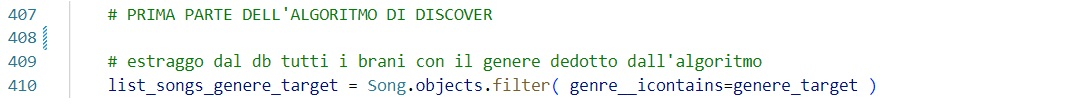
\includegraphics[scale=0.7]{images/alg2.jpg}
    \caption{Pseudocodice}
    \label{fig-pseudocodice-2}
\end{figure}
\vspace{1.5cm}

%algoritmo2
\begin{algorithm}[H]
    \caption{Step 2 - Brani}
    \SetAlgoLined
   
    \SetKwProg{myalg}{algoritmo}{ begin}{end}
    \myalg{Discover($curruser\_gender$, $curruser\_age$)}{
        \BlankLine
        \BlankLine
        \textbf{...}
        \BlankLine
        \BlankLine
        \textbf{/* Estrazione dei brani con genere target */}\

        \textbf{do}{
            $songs\_list \leftarrow Songs.\underline{filter}(genere=genere\_target)$
        }
        \BlankLine
        \BlankLine
        \Return{song\_list}\
            
        \KwResult{Lista brani con genere target}
        \BlankLine
        \BlankLine
        \textbf{...}
        \vspace{0.5cm}
        %\label(alg:1)
    }
\end{algorithm}





\newpage
%pseudocodice 3
Pseudocodice parte che suggerisce amici con gusti simili. 
\begin{figure}[H]
    \centering
    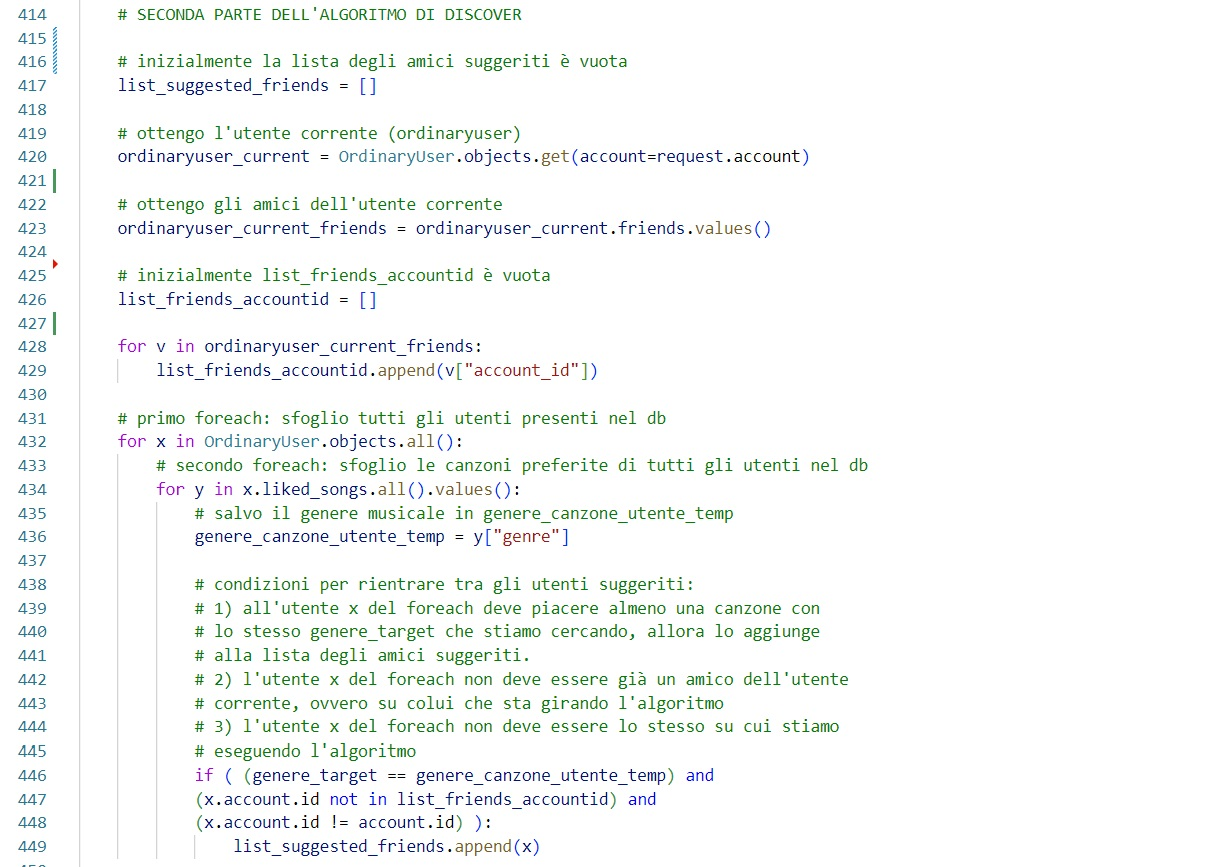
\includegraphics[scale=0.7]{images/alg3.jpg}
    \caption{Pseudocodice}
    \label{fig-pseudocodice-3}
\end{figure}


%algoritmo 3
\begin{algorithm}[H]

    \caption{Step 3 - Amici}
    \SetAlgoLined
   
    \SetKwProg{myalg}{algoritmo}{ begin}{end}
    \myalg{Discover($curruser\_gender$, $curruser\_age$)}{
        \BlankLine
        \BlankLine
        \textbf{...}
        \BlankLine
        \BlankLine
        \textbf{/* Creazione lista vuota */}\\
        \textbf{do}{
            $[] \leftarrow list\_suggested\_friends $
        }

        \BlankLine
        \BlankLine

        \textbf{/* Memorizzazione utente corrente */}\\
            \textbf{do}{
            $curr\_user \leftarrow curr\_user.\underline{get}()$
        }
        \BlankLine
        \BlankLine

        \textbf{/* Memorizzazione della lista di amici dell'utente corrente */}\\
        \textbf{do}{
            $friends\_id \leftarrow curr\_user.friends.\underline{values}() $
        }

        \BlankLine
        \BlankLine
        \textbf{/* Creazione lista vuota */}\\
        \textbf{do}{
            $[\ \ ] \leftarrow list\_user\_friends $
        }


        \BlankLine
        \BlankLine
        \For{v in friens\_id }{
            %\tcp{Blocco di istruzioni da eseguire per ogni valore di i}
            $list\_user\_friends.\underline{append}(v[id])$
            
        }
        \BlankLine
        \Return{risultato}\;

        \textbf{/* Memorizzazione amici dell'utente corrente */}\\
        \ForEach{ x in user.\underline{all}()}{
            %\tcp{Blocco di istruzioni per ogni elemento}

            \ForEach{y in x.liked\_songs.\underline{all}().\underline{values}()}{
                %\tcp{Blocco di istruzioni per ogni elemento}
                $genere\_temp \leftarrow y [genere] $\\
                \BlankLine
                \If{genere\_target = genere\_temp AND x.account.id != account.id AND x.account.id not in list\_user\_friends }{
                    %\tcp{Blocco di istruzioni se la condizione è vera}
                    list\_suggested\_friends.\underline{append}(x)
                }
                \BlankLine
            }
            \BlankLine
        }
    \BlankLine
    \Return{list\_suggested\_friends}\
    \BlankLine
    \BlankLine
    \KwResult{Lista utenti con gusti affini all'utente}
    \BlankLine
    \BlankLine
    \textbf{...}
    \vspace{0.5cm}
    %\label(alg:1)
    }
\end{algorithm}


\newpage
% pseudocodice 4
Pseudocodice parte finale algoritmo. 
\begin{figure}[H]
    \centering
    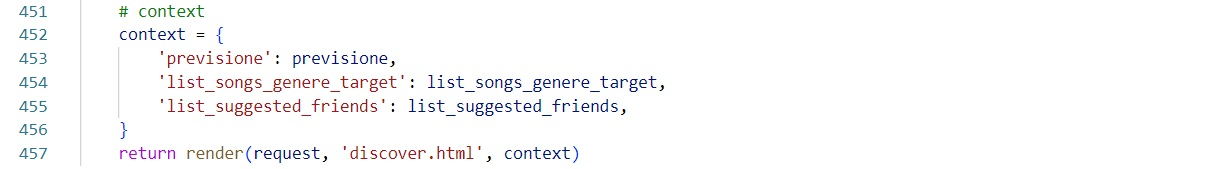
\includegraphics[scale=0.7]{images/alg4.jpg}
    \caption{Pseudocodice}
    \label{fig-pseudocodice-4}
\end{figure}
\vspace{0.5cm}

% algoritmo 4
\begin{algorithm}[H]

    \caption{Step 4 - Parametri di ritordno}
    \SetAlgoLined
   
    \SetKwProg{myalg}{algoritmo}{ begin}{end}
    \myalg{Discover($curruser\_gender$, $curruser\_age$)}{
        \BlankLine
        \BlankLine
        \textbf{...}
        \BlankLine
        \BlankLine
        \textbf{/* Ritorno parametri di interesse */}\\
        \Return{song\_list}\\
        \Return{list\_suggested\_friends}\\    
        \BlankLine
        \BlankLine
        \KwResult{Lista brani con genere target e lista utenti con gusti affini all'utente }
        \vspace{0.5cm}
        %\label(alg:1)
    }
\end{algorithm}






\newpage
\subsection{Analisi della complessità}
Per valutare la complessità temporale dell'algoritmo, vengono esaminate le operazioni principali che 
vengono eseguite e e viene analizzato come queste operazioni dipendono dalla dimensione dell'input. 
Di seguito viene fornita una stima approssimativa della complessità temporale per ogni parte dell'algoritmo:
\begin{itemize}
    \item \textbf{Lettura del file CSV:} La lettura del file CSV tramite la funzione $read\_csv$ ha una 
        complessità temporale che dipende dalla dimensione del file, nello specifico dal numero di righe e colonne del file.
        Supponiamo che ci siano n righe e m colonne nel file. La lettura del file richiede un'operazione 
        perogni cella nel file, di conseguenza la complessità è dell'ordine 
        di ${O(n*m)}$.
    \item \textbf{Creazione e addestramento del modello di classificazione:} La creazione del modello 
        \textit{DecisionTreeClassifier} e l'addestramento del modello tramite il metodo \textit{fit} dipendono dal numero di 
        caratteristiche e dal numero di esempi nel set di dati. Se denotiamo con d il numero di caratteristiche 
        e con k il numero di esempi, allora la complessità temporale può essere approssimata a $O(d * k log(k))$, 
        poiché la costruzione di un albero decisionale richiede operazioni che dipendono da entrambi i valori.
    \item \textbf{Previsione dei generi musicali:} La previsione dei generi musicali per l'utente corrente 
        utilizzando il modello addestrato ha una complessità temporale di ${O(1)}$, poiché si tratta di un singolo esempio
        (operazione costante).
    \item \textbf{Filtraggio dei brani musicali:} Il filtro dei brani musicali nel database attraverso la chiamata 
        a \textit{Song.objects.filter} può dipendere dal numero di brani nel database e dalla complessità della query. 
        Solitamente, questa operazione ha una complessità temporale dell'ordine di ${O(s)}$, dove s rappresenta il 
        numero di brani che soddisfano i criteri di filtro.
    \item \textbf{Ricerca degli amici suggeriti:} La ricerca degli amici suggeriti coinvolge \textit{due cicli for nidificati}. 
        Supponendo che ci siano \textit{n} utenti nel database e \textit{m} canzoni preferite per ogni utente, la complessità temporale di questa
        parte dell'algoritmo può essere approssimata a $O(n * m)$.
    \item \textbf{Creazione del contesto:} La creazione del contesto finale ha una complessità temporale trascurabile, 
        poiché coinvolge solo l'assegnazione di variabili.
    
     
\end{itemize}
Quindi, sommando tutte queste parti, possiamo dire che la complessità temporale complessiva dell'algoritmo è approssimativamente:

\boldmath
\begin{center}
    \BlankLine
    $O(n * m) + O(d * k log(k)) + O(s) + O(1)$
    \BlankLine
\end{center}
\unboldmath


È importante notare che questa stima approssimata dipende dal contesto specifico, dal volume dei dati e dalle 
operazioni effettuate. Per ottenere una stima più precisa, potrebbe essere necessario un'analisi dettagliata 
delle operazioni e delle strutture dati coinvolte nell'algoritmo.


\newpage
\subsection{Flowchart dell'algoritmo}
I passi base dell'algoritmo sono i seguenti: 

